\section{Global Motion Estimation}
\label{sec:02-gme}
When we look at a video, which corresponds to a sequence of images, called frames, we can spot the movement between one frame and the other by detecting the pixels that changed position with respect to the pair of frames.

This information can be encoded in a human-understandable format by presenting the needle diagram of the two frames; this kind of representation is shown in \cref{fig:needle-diagram}. 

\begin{figure}
    \centering
    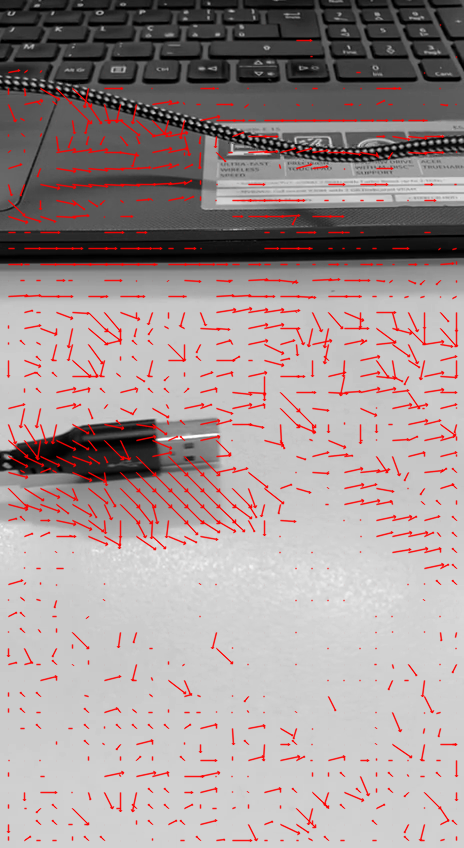
\includegraphics[width=.7\linewidth]{../assets/images/bbme-0-res.png}
    \caption{Needle diagram between two frames of a video sequence.}
    \label{fig:needle-diagram}
\end{figure}

The message of the figure is pretty clear: for each couple of frames we mark with an arrow the shift that the pixel has made. This gives us an indication of the actual movement of the recorded objects.

But the movement that we are able to extract from the two frames is what is usually called "apparent motion", which is a combination of two different factors:
\begin{itemize}[noitemsep]
    \item the global motion, which corresponds with the motion of the camera;
    \item the effective motion of the objects recorded.
\end{itemize}

An important task in computer vision is the global motion estimation, which corresponds to being able to distinguish these two different motions.
As stated in the abstract, this information is highly important for a number of applications, among which we find video coding, motion compensation and egomotion estimation.

But the task of distinguishing which movement is to be classified as global motion and which one is to be classified as object motion instead is not so easy. In fact, there is no clear feature that distinguishes the moving objects from the static background, and this leads to the need for complex tools to differentiate the two typed of motion.

The main approach to global motion estimation consists in ...


As \cite{Dufeaux2000}